\documentclass{article}

\usepackage[margin=1in]{geometry} 
\usepackage{amsmath,amsthm,amssymb,hyperref, multicol, tikz, romannum, wrapfig}
\usetikzlibrary{arrows.meta, positioning}
\usepackage[framemethod=tikz]{mdframed}



\newcounter{result}[section]
\setcounter{result}{0}



\newenvironment{result}[4]{
  \refstepcounter{result}

  \mdfsetup{
    frametitle={
      \tikz[baseline=(current bounding box.east),outer sep=0pt]
        \node[anchor=east,rectangle,fill=#4!20]
        {\strut #1~#2.\arabic{result}:~#3};
    },
    innertopmargin=10pt,
    linecolor=#4!20,
    linewidth=2pt,
    topline=true,
    frametitleaboveskip=\dimexpr-\ht\strutbox\relax
  }

  \begin{mdframed}\relax \begin{center}
}{
  \end{center} \hfill \end{mdframed} \vspace{3\baselineskip}
}

\hypersetup{colorlinks=True, linkcolor=cyan}



\newcommand{\R}{\mathbb{R}}  
\newcommand{\Z}{\mathbb{Z}}
\newcommand{\N}{\mathbb{N}}
\newcommand{\Q}{\mathbb{Q}}

\newcommand{\suc}{\!+\!\!+\!}


\begin{document}
\pagenumbering{arabic}


\title{Tao Analysis - My Visualisations and Proofs}
\author{Rhitt C}

\maketitle
\tableofcontents

\pagebreak

\setlength{\parskip}{8pt}
\section{Abstract and Motivation}

\subsection{Abstract}

I decided to write this text as a means to consolidate my personal understanding of undergraduate Real Analysis, 
and also to practise the skill of writing academic papers. 

It is heavily inspired and guided by Terrence Tao's Analysis Vol. \Romannum{1} and \Romannum{2}.
However, I have taken many liberties in altering formulations to my liking, 
completely spelling out motivating arguments before most definitions and theorems (even if this makes it clunky at times), 
going on large digressions, and providing visuals.
I'm also including my solutions to the exercises in Tao's texts, mainly for personal reference.

As a digression on expression, in aspiration of approbation from Big M's appellation upon examination, the language register is largely formal in an attempt to adhere to writing conventions. But we undergo register shifts towards 
informality where appropriate, particularly in avoiding the infamous passive voice\footnote{why is this even a scientific convention smh ts pmo}. This is because it would unnecessarily restrict syntactic freedom 
in a situational context where it is the \textit{content} that matters far more than the expression. Thus, it is more favourable to be able to convey the content precisely and elegantly without jumping though linguistic hoops every step of the way.

\subsection{Why do Analysis? - Motivation 1}
The motivation for Analysis is twofold:

Firstly, the most obvious reason is to understand deeper concepts that stray far from the base intuition you get from VCE and high school in general.
For example, you may have heard the result that there are more $x\in\R$ with $x\in(0, 1)$ than there are $p\in\Q$ with $p\in(-\infty, \infty)$\footnote{the precise statement is with a concept called \textit{cardinality}}.
Your intuition tells you this is absurd, because clearly both are infinite! How can we have $\infty_1>\infty_2$?
Even more counterintuitive is that there are \textit{just as many} $n\in\N$ as there are $x\in\Z$, even though clearly for every $n\in\N$ there are both $\pm n\in\Z$,
and so you'd expect there to be about twice as many integers as there are naturals.
It seems like mathematicians are just making stuff up at this point.
But in Real Analysis, we handle $\infty$ \textit{rigorously} to make such statements not only meaningful, but to fully understand the motivation for even discussing such matters in the first place.
The full level of rigour makes many theorems feel discoverable, in that you properly understand how you would derive and proof them in the first place.

We will see how it answers exactly what you can and can't do with $\infty$. E.g. Consider the matrix 
$$ M = \begin{pmatrix}
    1   & 0     & 0           & \cdots \\
    -1  & 1     & 0           & \cdots \\
    0   & -1    & 1           & \cdots \\
    0   & 0     & -1          & \cdots \\
    \cdots & \cdots  & \cdots & \ddots
\end{pmatrix} $$
You'd expect the sum of all elements $\sum M_{ij}$ to be the same either way, whether you sum over rows or over columns first.
But we have, if you'll excuse the lax notation, $$\sum_{\text{over rows first}} M = \sum_{\text{over columns}} \begin{pmatrix}1\\0\\0\\\vdots\end{pmatrix}=1,\qquad \sum_{\text{over columns first}} M = \sum_{\text{over rows}} \begin{pmatrix}0 & 0 & 0 & \cdots \end{pmatrix}=0$$
$$\therefore \left(\sum_{\text{over rows first}} M =1\right)\quad\neq\quad\left(\sum_{\text{over columns first}} M =0\right)$$

So we have illustrated that you can't always interchange the order in which you sum infinitely many numbers, contrary to intuition.
Real Analysis gives the full derivation for the precise conditions in which you can safely do so\footnote{see Fubini}.
As we have seen, it teaches you how to properly deal with $\infty$.
So in a sense, Real Analysis can make you like \textit{The Man Who Knew Infinity}\footnote{cold, cold, cold}.

More than that, Real Analysis answers to the highest echelon that is possible with logic (provably so, in fact) the \textit{why} behind essentially everything you've ever been taught in maths from kindergarten to high school, leave some small details about $\mathbb{C}$.
You realise the true degree of freedom that maths gives you.
And you learn complete objectivity.
You don't have to take anyone's word for it, just prove it yourself.
You learn to make a statement, and the proof of it, so damn precise that there is \textit{zero} ambiguity or subjectivity in it; I say this without hyperbole.
Doesn't matter if a teacher thinks your expression is lacking; you can be \textit{absolutely sure} that your statement is correct, given you're subtle enough with what is meant by correct.

\subsection{Why do Analysis - Motivation 2 (very important)}

Secondly, we will see how blindly following the whims of what our intuition deems reasonable can very easily lead to contradiction. 
The many times that this occurred historically, there was great philosophical anguish about what assumptions to discard and what to keep, greatly impeding on mathematical progress. 

\begin{wrapfigure}{r}{0.1\textwidth} \centering 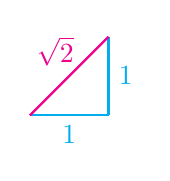
\begin{tikzpicture}
    \draw[cyan, thick] (0, 0) -- node[midway, below] {$1$} (1, 0);
    \draw[cyan, thick] (1, 0) -- node[midway, right] {$1$} (1, 1);
    \draw[magenta, thick] (1, 1) -- node[midway, left=5pt, above] {$\sqrt{2}$} (0, 0);
\end{tikzpicture} \end{wrapfigure}
For example, take $\sqrt{2}$, a quantity that arises in geometry very naturally as the length of the hypotenuse in a triangle with both other side lengths $1$.
In ancient Greece, many held the worldview that everything in the real world, like this hypotenuse, can be quantified as a rational number in $\Q$.
And they held this assumption to be so blatantly obvious that it underpinned their philosophy of everything from music to the universe itself.
So when it was found that $\sqrt{2}\in\Q$ would imply a contradiction, even though the triangle is very much real, it led to a crisis in which many ancient Greeks had to reevaluate their entire philosophy.

Because we've been taught from a young age that irrational numbers exist and do indeed show up in the real world, we now find the concept to be no doubt very intuitive. 
But how can we be absolute \textit{sure} that there isn't some other cancerous contradiction hiding somewhere in our mathematical foundations as well, just waiting to spread into everything we think we know, as it did for the Greeks?
The truth is, we're \textit{not} sure. And it's in fact been \textit{proven}\footnote{see G\"odel's Incompleteness Theorems} that we we can never be sure. 
Not unless we rob ourselves of the ability to do primary school arithmetic, which would be very absurd.

To be clear, the issue isn't with logic itself. As a rather lengthy aside, the question of whether logic is valid is philosophical in nature, and seemingly can't ever have a definitive resolution.
For example, it could very well be the case that we and our fictitious universe only exist in the incoherent dream of a butterfly. If so, logic as we perceive it only \textit{appears} valid to us,
yet completely wrong to a scientist observing the dream from outside in the real world. But even though such fundamental questions about reality may be interesting, 
doubting logic every step of the way puts overly restrictive bounds on what mathematical progress is possible.
So they're for the philosopher to ponder over. Instead, the mathematician prescribes a handful of obvious operations on True/False values, which formalises pure logic. E.g.
\begin{align*} &\text{(True }\&\text{ True) is True, but} \\ &\text{(True }\&\text{ False) is False, as True and False are said to contradict each other.} \end{align*}
Then they prescribe a few more rules on how to produce logical statements (with True/False value) from free variables (which can be mathematical objects), completing the formal link from maths to logic.
E.g.
\begin{align*} ((\forall x, P(x))\implies P(0)\text{) is True} \end{align*}
Finally, they combine all of this into what's very aptly named the formal grammar of logic. Confident that the grammar reflects reality, they hand it over to the philosopher to question the validity of.
The mathematician is now happy to accept this grammar as absolute and instead ponders questions about how the grammar of logic affects mathematical statements (theorems, lemmas, corollaries, etc.). 
And even if the philosopher someday finds evidence that the grammar is only valid in the dream of a butterfly and invalid outside of it, much of the work done by mathematicians could very well still be moulded to adhere to whatever rulebook is followed by the world outside the dream.

Now that we have a grammar for logic set in stone, how do we proceed?
The grammar can only tell us about the relationships between logical statements, but makes no comment about many individual statements involving free variables (more often than not the mathematical statements we are working with).
E.g. we can prove $$\text{(I am a lazy person \& all lazy people are monkeys)}\implies\text{(I am a monkey)}$$
as a whole is True directly from our grammar, but we can't individually show that (I am a lazy person) or (all lazy people are monkeys) are True with logic alone because of the free variables (I), (lazy person/people) and (monkey(s)).
And if either of those turn out to be False, then we have no information about whether (I am a monkey) is True or False. Thus, overall, we have a ($\implies$) statement that is True but we can't show definitely that (I am a monkey) \dots which is a good thing because I'm pretty confident I'm not a monkey (but can I \textit{show} definitively that I'm not? Once again, no). 

This is a necessary tradeoff we deliberately made to establish a barebone grammar of logic the philosopher can't immediately object to.

So what do we do do? It's absurd to say we should consider almost every theorem ever made unprovable just because we can't show it to be definitively True; that would put us in the same position as the philosopher!
Instead, you guessed it, we do the next best thing and instead show the truth of a ($\implies$) statement as follows: if we accept a base set of assumptions, which we call our \textit{axioms}, then the result we're trying to prove is True.

E.g. if we want to prove the statement that ($\forall x \in \N, x+1\neq0$), instead of showing its definitive truth (which is impossible), 
we instead show with a series of arguments that follow our logical grammar that
$$Axiom_1\;\&\;Axiom_2\;\& Axiom_3\;\&\;\dots\quad\implies\quad (\forall x \in \N, x+1\neq0)$$
and consider that sufficient to call it ``proven''. 

Of course, it's possible that neither a statement nor its negation can be implied from our axioms like that.
In such a case, the statement is called ``independent''.

\hfill

In summary, we do not deny the value of intuition. In fact, intuition is absolutely essential for \textit{developing} a conjecture and motivating why it might be plausible. 
Without it we are stuck running a fool's errand of perpetual guess and check, never able to come up with something original and useful.
But once we are confident that our conjecture is indeed plausible, we \textit{need} to follow a gold standard of proof. It's the only way to minimise the chance as much as feasible 
for a contradiction to sneak up on us from a single conjecture somewhere down the line. 
That would shatter the foundations of mathematics, much like it did for the Greeks when it was shown that $\sqrt{2}\in\Q$ is contradictory. The gold standard we set is:
\begin{result}{Definition}{D}{The Gold Standard of Proof}{green}
    A conjecture $C$ is considered "proven" under an axiomatic system $A_1\&A_2\&A_3\&\dots$ \textit{if and only if} we can show the following under our logical grammar

    $A_1 \& A_2 \& A_3\& \dots \implies C$
\end{result}

\pagebreak

\section{Construction of $\N$}


\subsection{Peano Axioms}

We lay our assumed Peano Axioms that relate to $\N=\{0, 1, 2, \cdots\}$, motivated by the construction of $\N$ as an analogue for the physical intuition of ``counting numbers". 
In doing so, we implicitly rely on some set theory, namely some of what is termed the ZFC Axioms of sets, which will be explored in the next chapter\footnote{This is so that the formulation of the Axiom of Infinity can be in terms of $\N$ and is thus much more intuitive. 
Rest assured, while the Peano Axioms refer to $\N$, they do not themselves make reference to the Axiom of Infinity, so there's no circularity. 
The standard in the literature is to merge the 5 Peano Axioms with our formulation of the ZFC Axiom of Infinity to yield a singular, strong and concise formulation of Axiom of Infinity, so ZFC can stand on its own as the foundation of modern maths. This will be explored briefly in the next chapter as a further digression on pure vs impure set theory than that of Tao's.}.
The Peano and ZFC Axioms are our \textit{only} assumptions in all of Analysis.

We shall see that this is sufficient for a very rich set of results about $\N, \Z, \Q, \R$ and some even more general statements\footnote{About all structures isomorphic to the ones mentioned, and also much later on, all metric spaces} to follow directly by formal logic from these foundational axioms, given relevant definitions.
In fact, almost all of modern maths relies on no more than the 8-9 ZFC and 5 Peano Axioms.
As I'm sure you'll agree after seeing how intuitive the axioms really are, this is quite a remarkable development in modern maths.
Motivated by these far-reaching implications of the Peano and ZFC Axioms, we set spelling out how a statement follows from these axioms as the gold standard for proof in modern maths.

We will see how blindly following the whims of what our intuition deems reasonable can very easily lead to contradiction. 
The many times that this occurred historically, there was great philosophical anguish about what assumptions to discard, greatly impeding on mathematical progress. 
For example, take $\sqrt(2)$, a quantity that arises in geometry very naturally as the length of a diagonal in a square with side length $1$.
When a proof arose that $\sqrt(2)$ could not be expressed as a fraction in simplest terms, it caused great distraught for the ancient Greeks.



\hfill

    We start with the bare minimum by demanding that some fixed object, namely $0$, be well defined. $0$ will be crucial to defining a few later axioms, as it gives us a sort of starting point.

    \begin{result}{Axiom}{P}{Existence of 0}{red}

        There exists an object $0$ that is natural and can be used in later axioms.
        $$\exists0\in \N \quad s.t.\quad \text{\textcolor{magenta}{P.3} and \textcolor{magenta}{P.5} are met.}$$

        
\begin{tikzpicture}[scale=1.2]
            \fill[cyan] (0,0) circle (3pt);
            \draw[ultra thick, cyan] (0,-0.2) -- (0, 0.2);
            \node[below, cyan, font=\large] at (0,-0.2) {$0$};
        \end{tikzpicture}

    \end{result}



    Now to populate $\N$, we introduce a new primitive operation (that will later by superseded by addition) called \textit{succession}, with the property of closure.
    Informally, we hope that it behaves like our intuition for incrementing a number by $1$, and thus forces the infinitely many ``counting numbers" to now be well defined and in $\N$.
    Denote the succession of all $n\in\N$ as $n\suc$, and label $(1:=0\suc),\; (2:=1\suc),\; (3:=2\suc),\;\dots$


    \begin{result}{Axiom}{P}{Closure of $\N$ under $(\suc)$}{red}
        All naturals have natural successions.
        $$\forall n\in\N\quad n \in \N \implies (n\suc) \in \N$$

        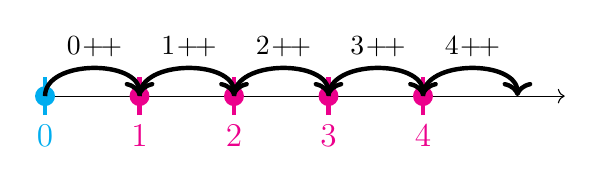
\begin{tikzpicture}[scale=1.2]

            \draw[->] (0,0) -- (5.5, 0);
            \fill[cyan] (0,0) circle (3pt);
            \draw[ultra thick, cyan] (0,-0.2) -- (0, 0.2);
            \node[below, cyan, font=\large] at (0,-0.2) {$0$};

            \fill[magenta] (1,0) circle (3pt);
            \draw[ultra thick, magenta] (1,-0.2) -- (1, 0.2);
            \node[below, magenta, font=\large] at (1,-0.2) {$1$};
            \draw[->, ultra thick] (0,0) to[bend left=90] node[pos=0.5, sloped, above] {$0\suc$} (1,0);

            \fill[magenta] (2,0) circle (3pt);
            \draw[ultra thick, magenta] (2,-0.2) -- (2, 0.2);
            \node[below, magenta, font=\large] at (2,-0.2) {$2$};
            \draw[->, ultra thick] (1,0) to[bend left=90] node[pos=0.5, sloped, above] {$1\suc$} (2,0);

            \fill[magenta] (3,0) circle (3pt);
            \draw[ultra thick, magenta] (3,-0.2) -- (3, 0.2);
            \node[below, magenta, font=\large] at (3,-0.2) {$3$};
            \draw[->, ultra thick] (2,0) to[bend left=90] node[pos=0.5, sloped, above] {$2\suc$} (3,0);

            \fill[magenta] (4,0) circle (3pt);
            \draw[ultra thick, magenta] (4,-0.2) -- (4, 0.2);
            \node[below, magenta, font=\large] at (4,-0.2) {$4$};
            \draw[->, ultra thick] (3,0) to[bend left=90] node[pos=0.5, sloped, above] {$3\suc$} (4,0);

            \draw[->, ultra thick] (4,0) to[bend left=90] node[pos=0.5, sloped, above] {$4\suc$} (5,0);

        \end{tikzpicture}
    \end{result}

    

    \pagebreak
    However, \textcolor{magenta}{P.1} and \textcolor{magenta}{P.2} alone are not strong enough to force $\N$ to populate with our infinitely many elements.
    In particular, they do not prevent existence of an $n\in\N$ with $n\suc=0$.
    And yet, informally speaking, this leads to a modulo cycle in which only $n+1$ elements exist in $\N$, and everything beyond that overflows back to $0$, like in a computer. 
    Modulo sets have many applications, but they are not what we desire as a full set of ``counting numbers'', particularly if that $n$ turns out to be $0$ itself, leading to a trivial $\N = \{0\}$.
    So we explicitly force $\N$ to not be such a modulo cycle by demanding that a natural's succession never overflows back to $0$.

    \begin{result}{Axiom}{P}{$\N$ is not a modulo cycle overflowing to $0$}{red}
        No natural's succession can be $0$.
        $$\forall n\in\N\quad (n\suc) \neq 0$$


        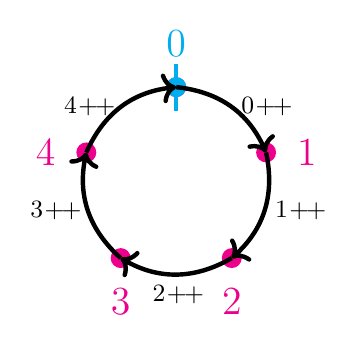
\begin{tikzpicture}[scale=1.2, every node/.style={font=\large, inner sep=1pt}]
            \def\n{5}
            \def\radius{1}

            \foreach \i in {0,...,4} {
                \pgfmathsetmacro{\angle}{90-\i*360/\n}
                \coordinate (N\i) at (\angle:\radius);
                \fill[magenta] (N\i) circle (3pt);
            }
            \fill[cyan] (N0) circle (3pt);

            \draw[ultra thick, cyan] (N0 |- 0,0.75) -- (N0 |- 0,1.25);

            \node[above=10pt, cyan, font=\Large] at (N0) {$0$};
            \node[right=10pt, magenta, font=\Large] at (N1) {$1$};
            \node[below=10pt, magenta, font=\Large] at (N2) {$2$};
            \node[below=10pt, magenta, font=\Large] at (N3) {$3$};
            \node[left=10pt, magenta, font=\Large] at (N4) {$4$};

            \draw[->, ultra thick] (N0) to[bend left=30] node[midway, right, outer sep = 1mm, font=\small] {$0\suc$} (N1);
            \draw[->, ultra thick] (N1) to[bend left=30] node[midway, right, outer sep = 1mm, font=\small] {$1\suc$} (N2);
            \draw[->, ultra thick] (N2) to[bend left=30] node[midway, below, outer sep = 1mm, font=\small] {$2\suc$} (N3);
            \draw[->, ultra thick] (N3) to[bend left=30] node[midway, left, outer sep = 1mm, font=\small] {$3\suc$} (N4);
            \draw[->, ultra thick] (N4) to[bend left=30] node[midway, left, outer sep = 1mm, font=\small] {$4\suc$} (N0);
        \end{tikzpicture}

    \end{result}


    As it stands, the issue hasn't been fully resolved yet.
    There is still the pathological case of an \textit{offset} modulo cycle, in which an $n\in\N$ overflows back so that $n \mapsto m\suc$ even though we already have a previous $m\mapsto m\suc$.
    We now complete our requirements on $(\suc)$ by demanding no such dual mappings to the same succession i.e. we make $(\suc)$ \textit{injective}.


    \begin{result}{Axiom}{P}{$\N$ has no otherwise offset modulo cycles either}{red}

        Succession is injective (one-to-one). That is, distinct naturals have distinct successions.
        $$\forall n, m\in\N\quad n \neq m \implies (n\suc) \neq (m\suc)$$

        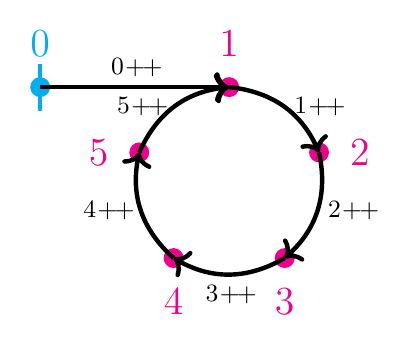
\begin{tikzpicture}[scale=1.2, every node/.style={font=\large, inner sep=1pt}]
            
            \def\n{5}
            \def\radius{1}

            \foreach \i in {0,...,4} {
                \pgfmathsetmacro{\angle}{90-\i*360/\n}
                \coordinate (N\i) at (\angle:\radius);
                \fill[magenta] (N\i) circle (3pt);
            }
            \fill[cyan] (-2, 0 |- N0) circle (3pt);
            \draw[ultra thick, cyan] (-2,0.75) -- (-2,1.25);


            \node[above=10pt, cyan, font=\Large] at (-2, 0 |- N0) {$0$};
            \node[above=10pt, magenta, font=\Large] at (N0) {$1$};
            \node[right=10pt, magenta, font=\Large] at (N1) {$2$};
            \node[below=10pt, magenta, font=\Large] at (N2) {$3$};
            \node[below=10pt, magenta, font=\Large] at (N3) {$4$};
            \node[left=10pt, magenta, font=\Large] at (N4) {$5$};

            \draw[->, ultra thick] (-2, 0 |- N0) to node[midway, above, outer sep = 1mm, font=\small] {$0\suc$} (N0);
            \draw[->, ultra thick] (N0) to[bend left=30] node[midway, right, outer sep = 1mm, font=\small] {$1\suc$} (N1);
            \draw[->, ultra thick] (N1) to[bend left=30] node[midway, right, outer sep = 1mm, font=\small] {$2\suc$} (N2);
            \draw[->, ultra thick] (N2) to[bend left=30] node[midway, below, outer sep = 1mm, font=\small] {$3\suc$} (N3);
            \draw[->, ultra thick] (N3) to[bend left=30] node[midway, left, outer sep = 1mm, font=\small] {$4\suc$} (N4);
            \draw[->, ultra thick] (N4) to[bend left=30] node[midway, left, outer sep = 1mm, font=\small] {$5\suc$} (N0);
        \end{tikzpicture}


    \end{result}


    \pagebreak 
    We now lay out by far the most useful axiom of $\N$ to handle the sheer infinite size of $\N$ recursively.
    It is induction.
    \begin{result}{Axiom}{P}{(PMI) Principle of Mathematical Induction}{red}
    
        If a proposition of naturals is met for $0$ (Base Case), and it being satisfied for some natural implies it's met for the succession as well (Inductive Case), then as a domino effect, then the proposition is met for all naturals.

        \hfill

        $\forall P:\N\to \{\text{True}, \text{False}\}\qquad(P(0)\;\&\;(\forall k\in\N)P(k)\!\!\implies\!\!P(k\suc)) \quad \implies \quad \forall n\in\N \quad P(n)$

        \vspace{2\baselineskip}

        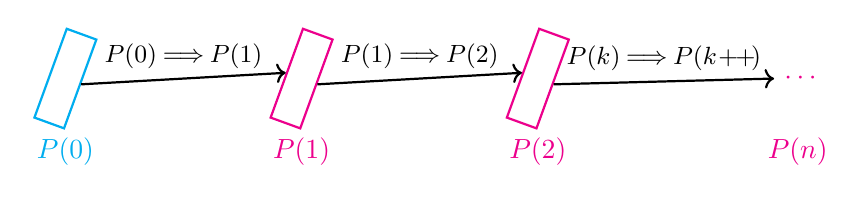
\begin{tikzpicture}[
            dom/.style={rectangle, draw, rotate=-20, minimum width=0.4cm, minimum height=1.2cm, thick},
            arrow/.style={->, thick}
        ]

            \node[dom, cyan] (D1) at (0,0) {};
            \node[below=18pt, cyan] at (D1) {$P(0)$};

            \node[dom, magenta] (D2) at (3,0) {};
            \node[below=18pt, magenta] at (D2) {$P(1)$};

            \node[dom, magenta] (D3) at (6,0) {};
            \node[below=18pt, magenta] at (D3) {$P(2)$};

            \node[below=18pt, magenta] at (9.3, 0) {$P(n)$};


            \draw[arrow] (D1.east) -- node[midway, above, font=\small] {$P(0)\!\!\implies\!\!P(1)$} (D2.west);
            \draw[arrow] (D2.east) -- node[midway, above, font=\small] {$P(1)\!\!\implies\!\!P(2)$} (D3.west);
            \draw[arrow] (D3.east) -- node[midway, above, font=\small] {$P(k)\!\!\implies\!\!P(k\suc)$} (9, 0) node[magenta, right] {$\cdots$};

        \end{tikzpicture}

    \end{result}

    Abstractly speaking, all sets $X$ equipped with an analogous operation $S: X\to X$ (refered to together as an algebraic structure $(X, S)$), that obeys the 5 Peano Axioms is said to be \textit{isomorphic} with $(\N, (\suc))$, denoted $(X, S)\cong(\N, (\suc))$.
    Note that due to our later discussions only relying on logical implications from the axioms, which are met by $(X, S)$, the results we derive must apply to every such $(X, S)$, given we rewrite our definitions accordingly.
    As such, we do not strictly define a particular $(\N, (\suc))$, but rather refer abstractly to any such solution $(X, S)$ to Peano.
    So in a sense, the Peano Axioms lay out a kind of citizenship test, in which $(X, S)$ is considered a natural structure if and only if it passes, and it gets all the perks of being a natural citizen that we will now derive.

    There is one final assumption that must be

    \subsection{Addition}
    \subsection{Multiplication}

\end{document}